\chapter{Related Work}
\label{chap:RelatedWork}

\section{Extreme Programming and Test-Driven Development}
\subsection{Extreme Programming}
Extreme Programming (XP) is a light-weight methodology for
small-to-medium-sized teams developing software in the face of vague or
rapidly changing requirements \cite{Beck:00}. It take common-sense
principles and practices to extreme level.
\begin{itemize}
\item If code reviews are good, we'll review code all the time (Pair Programming). 
\item If testing is good, everybody will test all the time (unit testing),
  even the customers (Functional Testing).
\item If design is good, we will make it part of everybody's daily business
  (Refactoring).
\item If simplicity is good, we will always leave the system with the
  simplest design that supports its current functionality (the simplest
  thing that could possibly work).
\item If architecture is important, everybody will work defining and
  refining the architecture all the time (Metaphor).
\item If integration testing is good, then we will integrate and test
  several times a day (Continuous Integration).
\item If short iterations are good, we will make the iteration really,
  really short--seconds and minutes and hours, not weeks and months and
  years (Planning Game).
\end{itemize}

XP is an agile process including 12 practices of: Planning Game, Small
Releases, Metaphor, Simple Design, Testing, Refactoring, Pair Programming,
Collective Code Ownership, Continuous Integration, Forty-hour Week,
On-site Customer and Coding Standards. \cite{Beck:00} As Kent Beck said XP is
not from ground up but many good practices derived from previous software
development. In XP these 12 practices support each other and complement
each other's weakness.  (Figure \ref{fig:XPSupportNetwork} Excerpted from
P70 \cite{Beck:00})
\begin{figure}[ht] 
  \centering
  \includegraphics[width=0.8\textwidth]{figs/XPSupportNetwork.eps}
  \caption{XP Support Network}\label{fig:XPSupportNetwork}
\end{figure} 

A typical XP project starts from planning game. Release plans will be laid
out in the planning game. Each release will vary from several weeks to
several months but not over half a year. Customers or stake holders define
release scope and important or critical business components go first.
Because XP is aiming at building simple but works software the advanced and
not-necessary features will not be considered until demanded. This will
maximize the Return-on-Investment (ROI). Communication, simplicity,
feedback and courage are four values XP will provide. Communications between
customer and developer, coach and developer, inter-developers are
encouraged by XP practices such as on-site customer, metaphor, coding
standard, collective ownership and pair programming directly or indirectly.
Feedback and courage are provided by test-driven development, on-site
customer, pair programming and continuous integration.  Simplicity is the
theme of XP through the entire development.  XP is another kind of
iterative incremental development (IID). The release plan is iterative and
development in each release is iterative too. Iteration in development is
from user story that can last only several days. The task assignment is
done in stand-up meeting. \cite{Beck:00}

Management of XP is through metrics, coaching, tracking and intervention.
It has roles developers, customer, tester, tracker, coach, consultant and
big boss. These roles are responsible for smooth execution and balance
maintenance of all 12 XP practices. Though XP acknowledges that each
practice has its own weakness it is not feasible for a developing team to
tranfer to XP seamlessly. Don Wells \cite{Beck:00} commented that XP
adoption can be iterative:
\begin{enumerate}
\item Pick your worst problem.
\item Solve it in XP way.
\item When it is no longer your worst problem, repeat.
\end{enumerate}

As we already know XP consists of 12 practices. Many of them can exist
independently. Planning game can fit into other IID process. On-site
customer can be available to other process models such as water-fall model.
Among 12 XP practices Pair Programming (PP) and Test-Driven Development
(TDD) often exist independently. They are widely applied and studied by
software developers, educators and researchers.

\subsection{Pair Programming}
Pair programming is an Extreme Programming practice. In pair programming
two programmers sit side-by-side at one computer, continuously
collaborating on same design, algorithm, code or tests. One acts as the
driver who types at computer. Another one acts as the navigator who is
responsible for high-level tasks like over-viewing design strategy,
inspecting code being typed for typos, syntax errors, or defects. Roles in
pair programming are dynamic and they can be exchanged during the
programming session or rotated in different programming sessions. Also the
pairs can be dynamically formed in a developing team. Two people actively
work on the same programming task with continuous collaboration.

Pair programming takes the privilege of code inspection a.k.a. code review
to improve code quality. Even though design or coding errors still can
exist but they will not last long because driver has to explain what he or
she is doing to navigator which provides a chance for both parties to think
it over. It looks like resources are wasted in pair programming because two
developers are invested on tasks that can be done by a solo developer;
however, Laurie Williams's case study concluded that pair programming will
not double development effort. In her study paired programmers are only
15\% slower than two independent individual programmers but produced 15\%
fewer bugs.  The knowing fact is that test and debug cost will be much
higher than initial programming so it will be economically paid off,
especially when some team members have to leave.

In extreme programming pair programming serves multiple purpose. Programs
are written by driver and navigator such that code review is done
simultaneously. The duo continuously communicate for better solution and
everyone inspects other's work. If driver goes the wrong way it can be
adjusted quickly by navigator without committing more mistakes, for
instance, when driver is not creating a test case before implementation
navigator can point it out so that they stay on the right track. Since
driver and navigator are exchanged during development both parties know
code well and own it. In case one programmer has to leave the developing
team risk is minimized because other people can take his or her work
over easily. The other benefit of pair programming is that junior
programmer can be coached and knowledge can spread over in the
team.\cite{PPWiki}

\subsection{Test-Driven Development}
Test-Driven Development is another Extreme Programming practice that has
its own benefits alone like pair programming. It's both the developing
method and design tool in extreme programming. Often it is called
Test-First Design (TFD) or Test-First Programming (TFP) because of its
natures. It has two fundamental rules:
\begin{itemize}
\item Write new code only if an automated test has failed.
\item Eliminate duplication.
\end{itemize}

Development of TDD is iterative. Test and implementation are added
incrementally under these two rules. An iteration can be elaborated as
following \cite{TDDWiki}:

\begin{enumerate}
\item Write the test
\item Write the code
\item Run the automated tests
\item Refactor
\item Repeat
\end{enumerate}

TDD is on the ground of a universally agreed claim that testing is good
to software project success. If it is done perfectly there is no need to
have a coverage tool because system is always 100\% tested. It supports
simplicity since developers only need to write enough code to make test
pass. Refactoring happens at the end of each iteration. Also unit tests can
serve as executing documentation of system so that re-usability is
improved.

In TDD unit tests are supported by XUnit framework. It is brought up by
Kent Beck, Ward Cunningham and Ron Jeffries in 1996 \cite{XP96}. It has the
following structure \cite{Beck:03}:

\begin{enumerate}
\item Invoke test method
\item Invoke setUp first
\item Invoke tearDown afterward
\item Invoke tearDown even if the test method fails
\item Run multiple tests
\item Report collected results
\end{enumerate}

In recent years xUnit has already been ported to more than 30 language
supports such as JUnit for Java, PyUnit for Python, NUnit for C\#.NET,
PHPUnit for PHP, CPPUnit for C++, DUnit for Delphi etc. \cite{XPSoftware}
and it has becoming the de facto standard of unit testing in software
development. With xUnit the unit testing is shifted from quality assurance
specialists or customers to developers.

This framework modulates unit testing onto method level. All public methods
in object-oriented domain are testable with this framework. It moves unit
testing from customer-oriented functional testing to the combination of
developer-oriented unit testing and customer-oriented functional testing.
Once project is brought up for functional testing it is already in high
quality insured by unit testing.

Theoretically speaking it is possible to do TDD perfectly but it is not
feasible in reality. First, developers as human beings are not good at
executing these two rigid rules. Second, there exists many holes such that
it is either not possible to do unit testing to some code or practically
infeasible in some cases. For instance, private methods are not accessible
for test purpose unless developer exposes them; GUI or event-driven methods
are not testable because they need humans intervention to make it happen;
some operations like database accesses are very time consuming such that unit
testing will take long time to run. Because of these limitations developers
would  not be able to follow TDD rules perfectly as Kent Beck wished.

In extreme programming process TDD can be executed better because other
practices can support it as figure \ref{fig:XPSupportNetwork} shows. Pair
programming supports TDD because two brains are better on creating good
unit tests and navigator can inform driver if unit tests are not created
before implementation. Coach can help pairs to design unit testing in case
it is hard or infeasible to do unit testing. Continuous integration can
help developers be aware of some unit tests fail or there is no unit test
to some code.


\section{Test-Driven Development in Practice}
Test-Driven Development is an incremental software development methodology
that stresses on exhausitive unit testing by creating test cases before
code implementation. It's a design and implementation methodology but
testing.  It ends with a rich suite unit test cases and high quality code
as it promises. It appears very often in software development tutorial
workshops
(\cite{OsheroveWorkshop:04,ClarkwareWorkshop:04,BENUGWorkshop:04,AdaptionTddWorkshop,IntustrialLogicTddWorkshop}),
technical reports, journals (\cite{TestDrivenDotComArticles}) and
blogsphere (\cite{TestDrivenDotComWeblogs}). Also many commercial and
open-source supporting tools (\cite{TestDrivenDotComTools}) are developed
in recent years.

\subsection{Characteristics of Test-Driven Development}

\subsubsection{Disciplined Small Steps}
In TDD development is incremental and iterative. Developers only write a
small portion of a unit test, or just one assertation each time, and then
just write enough code to test pass. At the beginnig the test target does
not exist so it cannot pass compilation. For instance, before we create
class Stack for a stack implementation we create a test class called TestStack.

    \begin{verbatim}
    package com.stack;

    import junit.framework.TestCase;

    /**
     * Tests stack operations. 
     */
    public class TestStack extends TestCase {
    }
    \end{verbatim}

To test whether stack can report its emptiness correctly developer adds one
assertation only in the first iteration.

    \begin{verbatim}
      /**
       * Tests empty stack.
       */
      public void testEmptyStack() {
        Stack stack = new Stack();
        assertTrue("Test empty stack", stack.isEmpty());
      }
    \end{verbatim}

It is not runnable because Stack class is not created yet. After creates
dummy implementation or stub of Stack it still cannot be compiled because
isEmpty() is not provided.

    \begin{verbatim}
    package com.stack;

    /**
     * Implements a stack.
     */
    public class Stack {
      /**
       * Constructs a stack.
       */
      public Stack() {
      }
    }
    \end{verbatim}

To make it compile developer goes ahead to add method isEmpty() which just
returns a constant.
    \begin{verbatim}
      /**
       * Whether stack is empty.
       * 
       * @return True if stack is empty.
       */
       public boolean isEmpty() {
         return false;
       }
    \end{verbatim}

Now it compiles but test fails because isEmpty() method simply returns
false. To make test pass developer changes it to return true. Then he/she
can go ahead to add another assertation and test case. As we can see from
above example development pace is really small in TDD. Generally one
iteration or cycle lasts from 30 minutes to 5 minutes. It rarely grows to
10 minutes \cite{GaryPollice:03}. It is totally okay to just add
implementation stub or simply returns a constant value to fake 
implementation (p13 \cite{Beck:03}, p169 \cite{Astels:03}).

\subsubsection{Consistent Refactoring}
Refactoring is an important portion in Test-Driven Development, it the
second TDD rule. By definition, refactoring is a disciplined technique for
restructing an existing body of code, altering its internal structure
without changing its external behavior \cite{Refactoring}. To make it
simple and concise refactoring is to change a program's interal structure
without affecting its external behaviors. In TDD developers need to
consistently do refactoring to support growing test suite without leaving
implementation code badly structured. When we do TDD the first priority is
to get test pass and the next is to remove duplication \cite{Beck:03}.
These two steps fulfil a complete TDD cycle. "Make it run, make it right.''
p24 \cite{Beck:03} Using the above example we can refactor isEmpty()
method to return an instance variable instead of a constant.
    \begin{verbatim}
      private int size = 0;
      /**
       * Whether stack is empty.
       * 
       * @return True if stack is empty.
       */
       public boolean isEmpty() {
         return this.size == 0;
       }
    \end{verbatim}

Now we run TestStack it passes. The duplication can be either on test code
or production code. As long as you get all tests pass you are confident to
do refactoring because unit tests can ensure you will not commit
unrecoverable big mistake.

\subsubsection{Courage, Rapid Feeback and One Ball in the Air at Once}
Kent Beck thinks TDD is a way of managing fear during development
\cite{Beck:03}. Programmers are in fear in software development because the
requirements are not clearly stated, techniques are new, problems are hard
to solve, or there is no enough time to do a thorough design and review.
Fears happen more often to novice programmers but experienced programmers
have fears too because a smallest mistake may break the whole system.
Experience programmers are good at debugging and have better intuition on
finding and solving bugs than novice programmers. In TDD developers ``test
a little, code a little and repeat.''\cite{Beck:03} Test cases guard code
development and provide instant feedback. Since the incremental step is
small it is impossible to commit big mistakes. If test fails it is easy to
fix it too. In software development developers carry the baggage with
requirement, system structure design, algorithm, code efficiency,
readibility and communication with other code etc. According to Martin
Fowler it is like keeping several balls in the air at once (Page 215
\cite{Beck:03}).  In TDD you only keep one ball in the air at once and
concentrate on that ball properly. Developer only needs to make the test
pass without worrying it is a good or bad design in TDD. In refactoring
step developer only worries about what makes a good design. Keeping one
ball only in the air helps doing good job on every aspect.

\subsubsection{Always Working Code}
TDD developers maintain a comprehend unit test suite and all test pass at
the end of each TDD cycle. The developing system is always working to the
designated tasks represented by unit tests. Since all test cases are
created in the domain of xUnit framework they can be integrated together to
do continuous integration. A test bot or agent can be setup to run all
tests everyday or every few hours \cite{ContinuousIntegration}. It works
well especially in team software development or in case it is not feasible
for a developer to run all tests in development in time manner.

\subsection{Benefits of Test-Driven Development}
\subsubsection{100\% Code Coverage}
If it is done perfectly TDD should always yield 100\% code coverage
\cite{Beck:03,Jeffries:00} as figure \ref{fig:TestScores} shows (Excerpted
from page 139 \cite{Jeffries:00}).
 
\begin{figure}[ht] 
  \centering
  \includegraphics[width=0.8\textwidth]{figs/TestScores.eps}
  \caption{Unit Test Scores}\label{fig:TestScores}
\end{figure} 

In practical it is not feasible to maintain 100\% but TDD developers do
yield high code coverage. Boby George and Laurie Williams's study finds
that TDD developers' test cases achieved 98\% method, 92\% statement and
97\% branch coverage \cite{George:02}. The experiment was conducted on a XP
developing team with Pair Programming practice too. Another study conducted
by Matthias M\"uller and Oliver Hagner in University of Karlsruhe found
that TDD developers yielded 74\% median branch coverage \cite{Muller:02}.
It's quite surprising because it is even lower than control group without
doing TDD whose median coverage is 80\%. On the fact that it is impossible
or not necessary to achieve 100\% this test coverage is still low. 

\subsubsection{Regression Test}
One principle of TDD is to create a regression unit test if system breaks.
The test fails first just as a typical TDD iteration. Code isolation is
another TDD principal that reduces coupling between objects. High CBO is
bad in object-oriented programming from modular design and reuse point of
views \cite{CKMetrics}. It's also straight forward the coupling can not be
zero because differant parts have to interact to make the system work. In
TDD developers run all tests regressively to make sure the new change will
not break other parts. Speaking in Java all package should have class
\verb!TestAll!  which assemblies all unit tests in the same package
together. When developer is working she or she just focus on tests in this
small area. XP has another practice called continuous integration to
execute all unit tests in timely manner to check system's consistency. If
the new change breaks system developer will know it in a few hours or a
day. A byproduct of TDD is a very comprehensive and exhaustive test set
that can serve as regression test suite.
 
\subsubsection{Executable Documentation}
In TDD there is no stacked written design documentations instead of
executing design documentation in unit tests. They are system-level
documentation and show how developers intended for the class to be used
\cite{ObjectMentorTDD,Ambler:03}.

\subsubsection{Clear Design}
XP community argues that TDD is not about test but design \cite{North:01}.
There is no big up-front design in XP and TDD but small incremental change.
Design decision is made incrementally by refactoring. Developers do
incremental change to the current code base instead of following design
documentation. Jim Little concluded that this evolutionary design yields
better results than big up-front design \cite{Little:01}. The design
architecture with upfront design generated a five-layer structure for data
persistence which is too complex in practice and the developing team was
completely lost. Intead the evolutionary is easy and effective in
architecture design. Also, TDD developer will not do anything extra except
for passing unit tests. It makes clean code that works \cite{Beck:03} and
is testable.

\subsubsection{High Quality Code}
Probably the most significant benefit of TDD to software development is
high code quality. Generally speaking TDD developers write code with high
coverage and the software created with TDD is more reliable than non-TDD
approach. Matthias M\"uller and Oliver Hagner's experiment in University of
Karlsruhe found that Test First Group (TFG)'s program has higher reliabilty
than controll group's code. In their experiment five TDD developers achieve
reliability over 96\% compared to only one program from the control group
that achieved this\cite{Muller:02}. Using black box test as external
validation TDD pairs passed approximately 18\% more black box tests in case
study conducted by Boby George and Laurie Williams \cite{George:03}.

\subsubsection{Increased Productivity}
TDD is faster test-last and code-N-fix. In TDD, testing is part of the
design process, it doesn't take long time to write a small test
\cite{MemoRandaBlog}. It is faster than test-last because developers need
to spend same amount or more time on creating tests after implementation.
Boby George and Laurie William's study showed that TDD developer spent 16\%
more than controller group but controller group did not primarily write any
worthwhile automated test cases though there were instructed to do so. TDD
code is much more reliable and with high code coverage. Since code is less
buggy it will save a lot time on debugging and maintenace.
\begin{quote}
``I have spent enough time in my career on silly bug-hunting, with TDD those
days are gone. Yes, there are still bugs, but they are fewer and far less
critical'' -- Thomas Eyde \cite{ExtremeJSBlog}
\end{quote}

\subsection{Barriers of Test-Driven Development}
More and more developers turn to TDD and many comercial and free workshops
are provided to evangelize TDD
\cite{TestDrivenDotComWeblogs,TestDrivenDotComArticle}.  Also, many tools
are created to support TDD \cite{TestDrivenDotComTools}. But still, many
developers are reluctant to TDD or even to give it a serious try despite on
the claim that TDD is infective \cite{Beck:03,TestInfected,EichertBlog,MasonBlog}. 
\subsubsection{Testability}
Darach Ennis argued that there are a lot of fallacies blowing around
various engineering organization and among various engineers \cite{Beck:03}. 
\begin{quote}
\begin{itemize}
\item You can't test GUIs automatically (e.g. Swing, CGI, JSP/Servlets/Struts)
\item You can't unit test distributed objects utomatically (e.g., RPC and Messaging style, or CORBA/EJB and JMS)
\item You can't test-first develop your database schema (e.g. JDBC)
\item There is no need to test third party code or code generated by external tools
\item You can't test first develop a language compiler/interpreter from BNF
  to production quality implementation.
\end{itemize}
\end{quote}

Most of these arguments are still valid but some operations are testable
nowadays. JSP and servlets can be tested by HttpUnit\cite{HttpUnit} or
Cactus\cite{Cactus}.  Mock object and Easy Mock can be used to test some
complex operations by providing fake implemention to the real system
\cite{MockObject}.

\subsubsection{Too Much Tests}
TDD is about design. To implement a task or user story developer makes a
list of test cases and maintains it when code grows. When it is empty and
there is no more test case developers can think of, task is done. All code
comes with test and sometimes test code may be larger than production code.
Apparently developers need to spend time on tests which are not thought as
production from customer point of view. XP says that it saves money for
customers on debugging and maintance, which is still not proved yet. A
model about Return on Investment (ROI) of TDD was brought up by Matthias
M\"uller and Frank Padberg shows how TDD can pay off the investment on
test\cite{Muller:03}. So far there is still no case study on cost benefit
analysis on TDD yet.

\subsubsection{Small Steps and Time-Consuming}
In TDD developers make small step each time. There will have many context
swith between test code and production, also many IDE activities. Using
previous isEmpty() method as example.
    \begin{verbatim}
      /**
       * Whether stack is empty.
       * 
       * @return True if stack is empty.
       */
       public boolean isEmpty() {
         return false;
       }
    \end{verbatim}

It is such a trivial thing such that most developers can make it right
without having a failed test. Kent Beck's opinion is that you can write
test that encourages hundreds of lines of code and hours of refactoring but
the tendency of TDD is to have smaller steps over time. Some developers
switched to TDD when old method cannot work, on example is defect removing
in debug.

\subsection{Testing Techniques and Tools}
\subsubsection{XUnit and its Related Tools}
XUnit is the corner stone of TDD. It makes test very simple and test
automation possible. The variation of xUnit includes JUnit for
Java\cite{JUnit}, SUnit for Small Talk\cite{SUnit}, CPPUnit for
C++\cite{CPPUnit}, NUnit for C\#.NET\cite{NUnit}, VBUnit for
VB\cite{VBUnit}, PYUnit for Python\cite{PYUnit} etc.  There are also some
extention for JUnit to test some complex operation, for instance, HttpUnit
for web\cite{HttpUnit}, Cactus for Servlet\cite{Cactus}, and DBUnit for
database\cite{DBUnit}. A new test tool called TestNG is developed to
simplify unit test using annotation and configuration file \cite{TestNG}.

\subsubsection{Mock Object}

\section{Case Studies on Test-Driven Development}
E. Michael Maximilien and Laurie Williams assessed Test-Drive Development
at IBM in the development of a new IBM Retail Store Solutions
version.\cite{Maximilien:03} The initiation of TDD came from the fact that
defect rate of each revisions did not drop in Functional Verification Test
(FVT) though developers have rich domain knowledge. TDD was introduced to
the developing team to alleviate the recurrent quality and testing
problems.  In their study they found defect rate dropped by 50\% in FVT
whereas productivity was not affected.  They believe that the drop of
productivity by TDD was complemented by the adoption of Microsoft Project
Central project management tool. The byproduct of TDD is a substantial
suite of unit tests. They also made test automation be possible and tests
were exercised once a day with the integration support. They also verified
the moral of TDD -- "test-infected'' phrased by Erich Gamma\cite{Beck:03}.
Developers were positive on TDD and intended to continue using it in their
future development.

Boby George and Laurie Williams summarized their findings regarding to
Test-Driven Development in three trial experiments \cite{George:03}.  TDD
approaches yielded superior external code quality measured by a set of
black box tests. TDD developers' code passed 18\% more functional black box
tests than controlled groups' code. Their results also showed that TDD
developers took more time than controlled groups. Additionally controlled
group did not write worthwhile automated test cases, which makes the
comparison on productivity uneven. The projects created by TDD developers
have very high test coverage. The mean method coverage is 98\%, statement
coverage is 92\% and branch coverage is 97\%.

Another case study conducted by Matthias M. M\"uller and Oliver Hagner in
University of Karlstruhe to test development efficiency, resultant code
reliability and program understanding. They found that switching to TDD
does not improve productivity and the code will not be more reliable than
with TDD approach. The only improvement is on code reusability because
tests help developers to use method or interface correctly \cite{Muller:02}.

\section{Hackystat}
Hackystat is an in-process automated metric collection system designed and
built in Collaborative Software Development Laboratory in University of
Hawaii. The attached IDE and ANT build sensors can collect the development
activities including file editing, class creation, method addition and
deletion as well as software metrics like unit test invocations, build
invocations, dynamic object-oriented metrics and other metrics as well.
Using Hackystat rich software metrics can be collected automatically to
study the development process without much work effort involved.

\subsection{Software Metrics}
A software metric is a measure of some property of a piece of software or
its specification \cite{SoftwareMetricWiki:05}. Common software metrics
include source lines of code, object-oriented metrics such as number of
methods in a class, coupling between objects, number of children etc, and
other metrics like function points, bugs per thousand lines of code, code
coverage and so on. Software metrics are widely used in software process to
predict and manage software development. A famous word by Tom Demarco is
that you cannot control what you cannot measure in controlling software
development \cite{SoftwareMetricWiki:05}. Software metrics make software
development process be measurable and process improvement be feasible.  

Koch summarized that there are two sets of objectives of software metrics 
\cite{QPMetricsKoch} :
\begin{itemize}
\item Measures are needed to develop project estimates, to monitor progress
  and performance, and to determine if the software products are of
  acceptable quality.
\item To the software organizations measurement can be used to determine
  overall productivity and quality level, to identify performance trends,
  to better manage software portfolios, to justify investments in new
  technologies, and to help planning and managing the software function. 
\end{itemize}

\subsection{Personal Software Process}
Personal Software Process (PSP) is a manual approach to record personal
software development activities to help project planning and estimation.
It's created and evangelized by Watt Humphrey at Software Engineering
Institute (SEI) in Carneige Mellon University. SEI provides a series of
training courses for developers and educator to grasp it \cite{Humphrey99}.
PSP has four levels range from 0 to 3 and the training course provides 10
programming exercises and five reports. On level 0 developers learn to
record their current practice using time recording log to understand how
time is spent to improve time usage. Other metrics like project size and
defects are measured too on level 0. On level 1 developers will do project
planning and estimation with the metrics data collected to improve
estimation accuracy. Code review and design review are introduced on level
2 to improve personal software quality. Level 3 is called cyclic personal
process. It suggests developers should divide large tasks into small pieces
to develop with PSP as Iterative Incremental Development (IID) advocates.

Many researches and experiments were conducted on PSP. Most of them show
that developers can improve productivity and reduce defect density with PSP
and the estimation accuracy is improved. Some researches reported poor
support for team software development and issue with data collection. Ann
Disney found that data entry is error prone in PSP.

\subsection{Automated Personal Software Process}
PSP helps individual developer to improve personal software process
maturity. To lower data entry overhead and improve PSP data quality.
Carleton A. Moore developed LEAP Toolkit in Collaborative Software
Engineering Laboratory in University of Hawaii. With LEAP Toolkit
developers can record their time and enter data easily. It improves data
accuracy and provides regression analyses that cannot be done manually in
PSP \cite{csdl-99-15}.

\subsection{Hackystat}
Tools like LEAP Toolkits make it fairly easy to record PSP data and conduct
project planning and estimation. In LEAP developers enter PSP data using
clock control and other data entry forms but developers will have to stop
their on-hand work often to input data, which reduces its effectness on
process improvement, project planning and estimation. It is also hard to do
collaboration to support team project development. In 2001 Philip Johnson
etc started Hackystat project to collect development automatically.
Hackystat sensors can be installed in development environments such as
XEmacs, JBuilder, Eclipse and Visual Studio etc to collect software
development data unobtrusively. Hackystat sensors will send out metric data
collected to a centerized data server with SOAP protocol \cite{csdl2-04-05}
in a period-based fashion. Hackystat is extensible so that many kinds of
metrics can be collected except for time, size and defect measurement.
Most development activities such as opening file, editing file, closing
file and refactoring data can be collected by Hackystat sensors. Unit test
case exercises and test coverage can be recorded too by Hackystat. It
supports development collaboration by defining project with common
workspaces\cite{csdl2-04-05}. Initial case studies (\cite{csdl2-03-13},
\cite{csdl2-03-12}) found that Hacksytat has very low overhead for students
and Hackystat analyses are very helpful on student projects. Usage of
Hackystat on extreme programming, high performance computing, project
management and software reviews are being explored in Univeristy of Hawaii
and affiliate organizations.



















